%!TEX root = ../main.tex

\chapter{Conformance Testing} \label{chp:conformancetesting}    % a che serve, con specifica ambiente di sviluppo (python, poetry, git, gitlab DEI)
I test di conformità, come anticipato nella sezione \ref{sec:standard-mpai}, sono un insieme di attività di verifica che determinano l'aderenza di un processo, prodotto o servizio a dei requisiti tecnici o a delle norme.
Nel caso in esame, \ac{ARP}, si tratta di verificare che il suo funzionamento segua, entro certi limiti (necessari anche perchè è una IA), le specifiche tecniche. In \ac{MPAI}, questi test, sono definiti all'interno di un documento apposito.

L'obiettivo di questa tesi è quella di scrivere il codice dei test di conformità, basandosi sul documento che li descrive fornito da MPAI.

L'ambiente di sviluppo è un ambiente virtuale di \href{https://python-poetry.org/}{Poetry} basato su Python 3.10 (poi aggiornato a 3.11)\footnote{Vedi sezione \ref{ssec:py-311}}, su una macchina Windows 11 (per alcuni confronti, occasionalmente è stata utilizzata una macchina virtuale con Ubuntu 20.04.6 LTS). L'ambiente di produzione è un server Docker con container linux.\footnote{Per questo motivo l'implementazione del CSC ha anche una modalità di esecuzione come server con protocollo gRPC, utilizzato per fare comunicare i vari \acp{AIM} tra loro.} Per il versionamento del software viene usato \href{https://git-scm.com/}{git}, utilizzando come server il \href{https://gitlab.dei.unipd.it/}{GitLab del \ac{DEI}}.


\section{Tests e \acl{TDD}} \label{sec:tests-tdd}
Il software testing è il processo di valutazione e verifica del corretto funzionamento di un prodotto software rispetto alle aspettative; la creazione di test suites ha l'obiettivo di rilevare bug prima di rilasciare il prodotto.
Solitamente si tende ad automatizzare i test attraverso alcuni framework in modo tale da poterli eseguire ad ogni modifica del codice.

Il \acfi{TDD} è un approccio allo sviluppo di software che prevede la scrittura dei test prima di quella del codice ai quali deve esserne sottoposto; inoltre i test sono da ripetere man mano che il software viene sviluppato.
I test di conformità sono il documento ed i test stessi che l'implementazione software delle specifiche tecniche dovranno rispettare, quindi la loro scrittura e comunque una correzione del codice basandosi su di essi può essere riconosciuta come un approccio di \ac{TDD}. % TODO vedere se dare più importanza


\subsection{Pytest} \label{ssec:pytest} % funzionamento/utlità, xdist per parallelizzare, json-report per scrivere il report richiesto, fixtures per eseguire funzione per ogni file
Uno dei framework per il testing in Python più popolari è \href{https://pytest.org}{pytest}, esso permette di ottenere informazioni dettagliate sul fallimento degli \texttt{assert} statements\footnote{\texttt{assert} è la parola chiave che permette di effettuare i test, nello specifico il test procede se i suoi parametri sono \texttt{True}, mentre viene lanciato \texttt{AssertionError} se i suoi parametri sono \texttt{False}.}, di avere fixtures\footnote{Una \textit{fixture} è un elemento del software testing che viene utilizzato per definire un contesto per l'esecuzione di uno (o più) test.} modulari e di essere compatibile con numerosi plugin esterni.

\href{https://github.com/numirias/pytest-json-report}{pytest-json-report} è un plugin che è stato utilizzato per creare i report richiesti come output del conformance testing in formato JSON.

\href{https://pytest-xdist.readthedocs.io/}{pytest-xdist} è un plugin che è stato utilizzato per parallelizzare l'esecuzione (vedi sezione \ref{sec:parallelizzazione}

Sono state utilizzate delle fixture per definire l'ambiente di test e per ottenere delle cartelle di test (\verb|pytest_sessionstart|, \verb|pytest_sessionfinish| e \verb|tmp_path|), inoltre è stata parametrizzata l'esecuzione delle varie funzioni di test in modo tale da essere eseguite per ogni documento digitalizzato tramite il decoratore \texttt{@pytest.mark.parametrize}.


\section{\acs{CAE}-\acs{ARP} packager} \label{sec:test-packager}
Il primo \ac{AIM} preso in esame è stato il packager.

\begin{figure}[h]
    \centering
    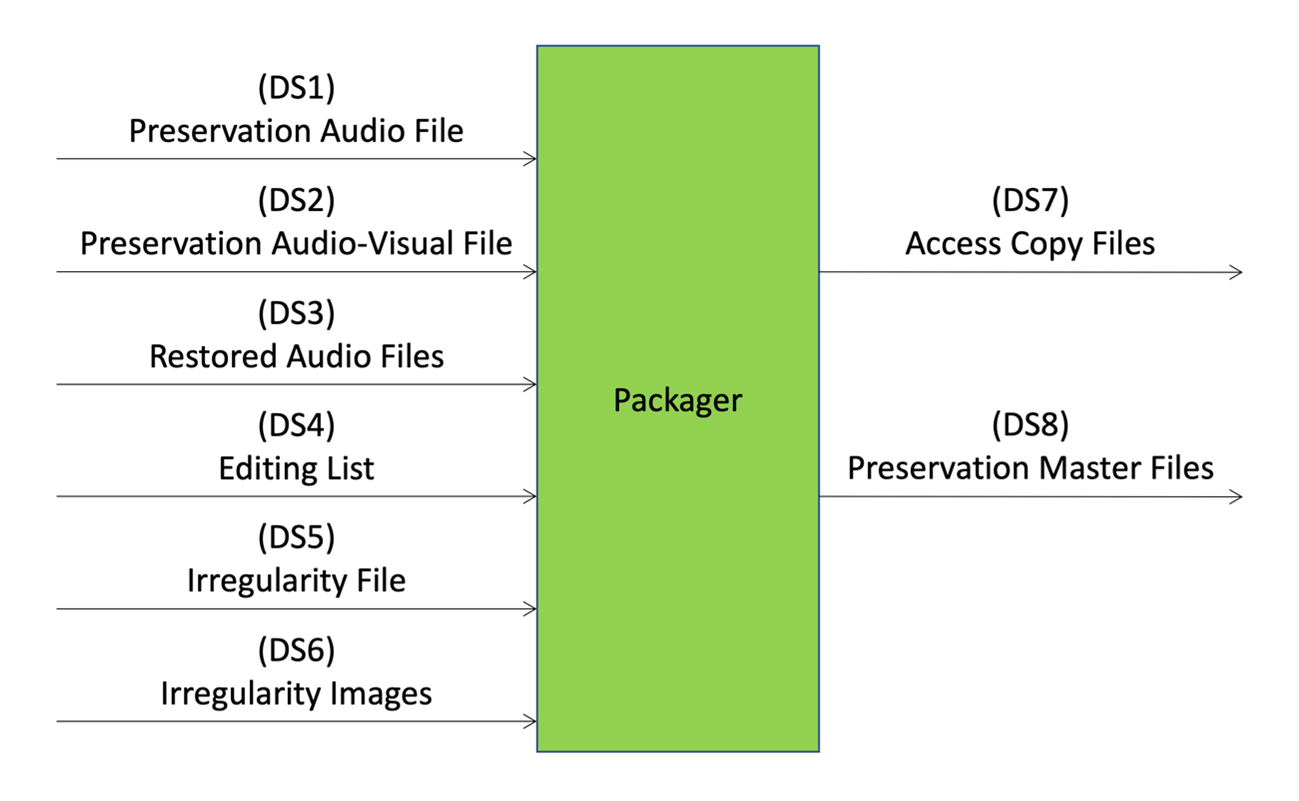
\includegraphics[width=0.9\textwidth]{packager.png}
    \caption{\ac{ARP} Packager}
    \label{fig:packager}
\end{figure}

% \begin{table}[h]
%     \centering
%     \begin{tabular}{|c|c|}
%         \hline
%         \textbf{Input data}             &   \textbf{Output Data}\\
%         \hline
%         Preservation Audio File         &   Access Copy Files\\
%         Preservation Audio-Visual File  &   Preservation Master Files\\
%         Restored Audio Files            &   \\
%         Editing List                    &   \\
%         Irregularity File               &   \\
%         Irregularity Images             &   \\
%         \hline
%     \end{tabular}
%     \caption{I/O di \ac{ARP} Packager}
%     \label{tab:packager-io}
% \end{table}

Il packager, come anticipato nella sottosezione \ref{ssec:mpai-cae-arp}, è l'ultimo \ac{AIM} ad essere eseguito e si occupa di raccogliere tutti i file elaborati e di restituire in uscita all'\ac{AIW} una cartella con la copia d'accesso dei file ed una con i file grezzi accompagnati da tutte le irregolarità trovate, vedi schema in figura \ref{fig:packager}.

Viene riportata la descrizione dei conformance tests da seguire, definita da MPAI, nella tabella \ref{tab:packager-valutazione}.\footnote{Estratta dalla versione WD 0.15.2 del documento MPAI Conformance Testing per \ac{CAE}.} 

\begin{table}[h]
    \centering
    \begin{tabular}{|p{0.2\textwidth}|p{0.8\textwidth}|}
        \hline
        \textbf{Means}   &   \textbf{Actions}\\
        \hline
        \textbf{Conformance Testing Dataset}    &
            DS1: n Preservation Audio Files.\newline
            DS2: n Preservation Audio-Visual Files related to DS1.\newline
            DS3: n Restored Audio Files arrays related to DS1 coming from Tape Audio Restoration.\newline
            DS4: n Editing Lists related to DS3 coming from Tape Audio Restoration.\newline
            DS5: n Irregularity Files related to DS1 coming from Tape Irregularity Classifier.\newline
            DS6: n Irregularity Images related to DS5 coming from Tape Irregularity Classifier.\newline
            DS7: n Access Copy Files.\newline
            DS8: n Preservation Master Files.\\
        \hline
        \textbf{Procedure}  &
            1.	Feed Packager under test with DS1, DS2, DS3, DS4, DS5 and DS6.\newline
            2.	Compare the output Access Copy Files with DS7.\newline
            3.	Compare the output Preservation Master Files with DS8.\\
        \hline
        \textbf{Evaluation} &
            For a given input tuple, verify that:\newline
                1.	The output Access Copy Files contain the Restored Audio Files, the Editing List, the Irregularity File and the set of Irregularity Images in a .zip file, and is therefore equal to DS7.\newline
                2.	The output Preservation Master Files contain the Preservation Audio File, the Preservation Audio-Visual File with the audio of the Preservation Audio File, the Irregularity File and the Irregularity Images, and is therefore equal to DS8.\newline
            An error on any of the output arrays will make the Packager under test not conformant.\\
        \hline
    \end{tabular}
    \caption{Test di conformità per \ac{ARP} Packager}
    \label{tab:packager-valutazione}
\end{table}

Ad ogni esecuzione dei test è richiesto di inserire i dati nella tabella \ref{tab:packager-report}.
\begin{table}[H]
    \centering
    \begin{adjustbox}{max width=\textwidth}
        \begin{tabular}{|c|c|}
            
            \hline
            Conformance Tester ID                       &   Unique Conformance Tester Identifier assigned by MPAI\\
            \hline
            Standard, Use Case ID and Version           &   Standard ID and Use Case ID, Version and Profile of the standard in the form “CAE:ARP:1:0”.\\
            \hline
            Name of AIM                                 &   Packager\\
            \hline
            Implementer ID                              &   Unique Implementer Identifier assigned by MPAI Store.\\
            \hline
            AIM Implementation Version                  &   Unique Implementation Identifier assigned by Implementer.\\
            \hline
            Neural Network Version (optional)           &   Unique Neural Network Identifier assigned by Implementer.\\
            \hline
            Identifier of Conformance Testing Dataset   &   Unique Dataset Identifier assigned by MPAI Store.\\
            \hline
            TestID                                      &   Unique Test Identifier assigned by Conformance Tester.\\
            \hline
            Actual output                               &   Actual output provided as a matrix of n rows containing output assertions.\\
                                                        &   \begin{tabular}{|c|c|c|c|c|}
                \hline
                Output                      &   Files                           &   1   &   \dots   &   n\\
                \hline
                Access Copy Files           &   Restored Audio Files            &   T/F &   \dots   &   T/F\\
                                            &   Editing List                    &   T/F &   \dots   &   T/F\\
                                            &   Irregularity File               &   T/F &   \dots   &   T/F\\
                                            &   Irregularity Images             &   T/F &   \dots   &   T/F\\
                \hline
                Preservation Master Files   &   Preservation Audio File         &   T/F &   \dots   &   T/F\\
                                            &   Preservation Audio Visual File  &   T/F &   \dots   &   T/F\\
                                            &   Irregularity File               &   T/F &   \dots   &   T/F\\
                                            &   Irregularity Images             &   T/F &   \dots   &   T/F\\
                \hline
            \end{tabular}\\
                                                        &   Final assertion: T/F\\
            \hline
            Execution time (optional)       &   Duration of test execution\\
            \hline
            Test comment (optional)         &   Comments on test results and possible needed actions.\\
            \hline
            Test Date                       &   yyyy/mm/dd.\\
            \hline
        \end{tabular}
    \end{adjustbox}
    \caption{Report da compilare ad ogni esecuzione del packager.}
    \label{tab:packager-report}
\end{table}
Il report viene compilato automaticamente in un file JSON per quanto conosciuto dal software anche grazie all'aiuto della libreria \href{https://github.com/numirias/pytest-json-report}{pytest-json-report} che raccoglie i risultati dei test in un formato machine-readable.

Il seguente listato ne è un esempio:
\lstinputlisting[language=json]{listings/packager-report.json}
% TODO inserire report riportato in tabella?


\subsection{Bug ed altri problemi pre-esistenti}    % moviepy vs ffmpeg (errori nel video e audio transcodifica in mp3), offset
Prima di dedicarsi alla scrittura dei test, si è verificata la corretta funzionalità del software.

Sono stati riscontrati dei problemi importanti relativi alla creazione del \textit{PreservationAudioVisualFile}

\begin{lstlisting}[language=Python, caption=Codice iniziale; creazione PreservationAudioVisualFile]
# Create Preservation Audio-Visual File with substituted audio
video_file = files_name + '.mov'
pvf_path = os.path.join(working_path, 'PreservationAudioVisualFile/', video_file)
try:
    audio = AudioFileClip(paf_path)
    video = VideoFileClip(pvf_path)
    # Open Irregularity File to get offset
    irregularity_file_json = open(
        os.path.join(temp_path, 'TapeIrregularityClassifier_IrregularityFileOutput2.json')
    )
    irregularity_file = json.load(irregularity_file_json)
    offset = irregularity_file['Offset']/1000
    if offset > 0:
        audio = audio.subclip(t_start=offset)
    else:
        video = video.subclip(t_start=offset)
    video = video.set_audio(audio)
    video.write_videofile(pmf_path + 'PreservationAudioVisualFile.mov', bitrate='3000k', codec='mpeg4')
    print("Preservation Audio-Visual File created")
except OSError:
    pprint(f"Preservation Audio-Visual File file '{pvf_path}' not found!", color=Color.RED)
    quit(os.EX_NOINPUT)
\end{lstlisting}

Il primo problema è relativo alla sincronizzazione del video con l'audio: l'audio deve essere anticipato se viene trovato un offset positivo, altrimenti deve essere anticipato il video.
Alle righe 12-16, si osserva che il comportamento non è quello richiesto, dato che a riga 16 l'offset ha valore negativo, allora \href{https://zulko.github.io/moviepy/}{MoviePy}, libreria utilizzata per eseguire editing video, farà iniziare la traccia a partire da $|offset|$ secondi prima del termine della clip.\footnote{Codice sorgente: \url{https://zulko.github.io/moviepy/_modules/moviepy/Clip.html#Clip.subclip}}    % TODO da verificare se vero

Il secondo problema è relativo alla non specifica nel codice della codifica audio che porta la libreria MoviePy a ricadere nel comportamento di default, ovvero generare un file con codifica MP3 (lossy) a \qty{44100}{\Hz} e ad avere di conseguenza, in questo caso, una transcodifica, il che non è ottimale per un software che ha come obiettivo la conservazione di documenti audio.

Il terzo problema invece è provocato dalla libreria \href{https://zulko.github.io/moviepy/}{MoviePy} che, per motivi sconosciuti e solo in alcuni casi, genera file corrotti nella traccia video, nello specifico che si bloccano dopo alcuni secondi.  % TODO verificare se c'entra con il problema di cui sopra.

Per risolvere questi due problemi si è scelto di sostituire MoviePy direttamente con \href{https://ffmpeg.org/}{FFmpeg}, ottenendo come risultato il seguente codice:
\begin{lstlisting}[language=Python, caption=Codice finale; creazione PreservationAudioVisualFile]
# Create Preservation Audio-Visual File with substituted audio
video_file = files_name + '.mov'
pvf_path = os.path.join(working_path, 'PreservationAudioVisualFile/', video_file)
try:
    # Open Irregularity File to get offset
    irregularity_file_json = open(
        os.path.join(temp_path, 'TapeIrregularityClassifier_IrregularityFileOutput2.json')
    )
    irregularity_file = json.load(irregularity_file_json)
    offset = irregularity_file['Offset']
    command_to_run = ['ffmpeg',
                      '-y', '-hide_banner', '-loglevel', 'error']
    # If offset is positive, the audio is anticipated, otherwise video is anticipated (through seek)
    if offset > 0:
        command_to_run = command_to_run + ['-i', pvf_path,
                                           '-ss', str(offset)+'ms', '-i', paf_path]
    else:
        command_to_run = command_to_run + ['-ss', str(offset * -1)+'ms', '-i', pvf_path,
                                           '-i', paf_path]
    command_to_run = command_to_run + ['-c:v', 'mpeg4', '-c:a', 'copy',
                                       '-map', '0:v', '-map', '1:a',
                                       '-b:v', '3M', '-maxrate', '4M', '-bufsize', '4M',
                                       pmf_path + 'PreservationAudioVisualFile.mov']
    subprocess.run(command_to_run)
    print("Preservation Audio-Visual File created")
except OSError:
    pprint(f"Preservation Audio-Visual File file '{pvf_path}' not found!", color=Color.RED)
    quit(os.EX_NOINPUT)
\end{lstlisting}


\subsection{Come verificare l'uguaglianza tra audio}  % fingerprinting con chromaprint, suo wrapper in python, free software e mie contribuzioni, comunicare col mantainer
Per verificare l'uguaglianza fra tracce audio, inizialmente si è provato un confronto tramite le librerie \textit{hashlib} o \textit{filecmp}, ma entrambi i test non hanno avuto successo perchè in alcuni casi non è richiesto di verificare che il file sia lo stesso identico (stesso hash), ma piuttosto di controllare che il suono sia il medesimo\footnote{La differenza si osserva, per esempio, quando si hanno 2 file, uno scostato di qualche secondo rispetto all'altro, questo è ciò che accade nel caso in esame, quando si esegue la sincronizzazione audio/video.}.

La soluzione trovata si basa sulla libreria \href{https://acoustid.org/chromaprint}{chromaprint}\footnote{chromaprint è la libreria che è alla base del progetto AcoustID, utilizzato nel piuttosto famoso software \href{https://musicbrainz.org/}{MusicBrainz} (\href{https://picard.musicbrainz.org/}{Picard}) che serve a taggare le proprie tracce musicali.}, la quale permette di ricavare delle impronte digitali (\textit{fingerprint}) da delle tracce audio, in maniera da poi confrontarle tra loro per ottenere la loro somiglianza.    % TODO taggare va bene?

È stata utilizzata in particolare una libreria Python, la quale non è altro che un wrapper di AcoustID, chiamata \href{https://github.com/beetbox/pyacoustid}{pyacoustid} che aiuta lo sviluppatore Python esponendo direttamente le API di chromaprint ed un metodo per confrontare le impronte.

\begin{lstlisting}[language=Python, caption=Test di comparazione di due file audio tramite la loro impronta digitale]
AUDIO_THRESHOLD = 0.7   # (ratio)
# [...]
input_fingerprint = acoustid.fingerprint_file(input_paf_path)
output_fingerprint = acoustid.fingerprint_file(output_paf_path)
assert acoustid.compare_fingerprints(input_fingerprint, output_fingerprint) > AUDIO_THRESHOLD, "PreservationAudioFile.wav is not the same as input"
\end{lstlisting}

Come si può leggere dal codice, è stata scelta come soglia di somiglianza il $70\%$, non è il $100\%$ perchè, ad esempio, nei casi in cui è stata effettuata la sincronizzazione audio/video l'audio non è esattamente uguale, inoltre dai vari test eseguiti sui dataset forniti, questo valore ha funzionato correttamente.

Durante la scelta della soglia da adottare sono state eseguite diverse prove ed è stato verificato che, correttamente, nel caso dei file in esame, si ottengono dei risultati elevai, talvolta uguali a $1$, mentre in caso di file diversi, si ottiene un valore tendente a $0$.\footnote{Alcune prove si possono trovare alla pagina: \url{https://github.com/albertopasqualetto/Tesi-triennale/blob/main/Notebooks/chromaprint_comparisons.ipynb}}   % non è più stata trovata una differenza in base al codec

La libreria pyacoustid, nelle prime fasi di scrittura dei test, non era ancora completamente funzionante e compresa del metodo per comparare le impronte digitali, infatti la sua versione 1.2.2, presente sulla repository \href{https://pypi.org/}{PyPi}, non vedeva ancora implementata la funzione \verb|compare_fingerprints|, già presente invece sulla sua repository GitHub grazie al contributo di un utente; tale implementazione era, però, non funzionante a causa di alcuni errori del codice come si può vedere dai cambiamenti applicati successivamente e descritti qui: 

\begin{lstlisting}[language=diff]
@@ -382,7 +382,7 @@ def _match_fingerprints(a: List[int], b: List[int]) -> float:
            if biterror <= MAX_BIT_ERROR:
                offset = i - j + bsize
                counts[offset] += 1
-    topcount = counts.max()
+    topcount = max(counts)
    return topcount / min(asize, bsize)


@@ -397,8 +397,8 @@ def compare_fingerprints(a, b) -> float:
        raise ModuleNotFoundError("function needs chromaprint")

    # decompress fingerprints
-    a = [int(x) for x in chromaprint.decode_fingerprint(a)[0]]
-    b = [int(x) for x in chromaprint.decode_fingerprint(b)[0]]
+    a = [int(x) for x in chromaprint.decode_fingerprint(a[1])[0]]
+    b = [int(x) for x in chromaprint.decode_fingerprint(b[1])[0]]
    return _match_fingerprints(a, b)
\end{lstlisting}

Per applicare queste modifiche è stato necessario effettuare una \href{https://github.com/beetbox/pyacoustid/pull/78}{\ac{PR}}\footnote{Una \ac{PR} è una richiesta ai manutentori del codice aggiungerne di proprio per implementare nuove funzioni o per correggere dei problemi.} sulla repository ufficiale a cui ha seguito uno scambio di messaggi con il manutentore e l'implementatore del codice; questa è una pratica comune nel mondo del software libero, il quale, tra i vari vantaggi, permette di leggere il codice sorgente e contribuire con dei miglioramenti alle tecnologie che si utilizzano.\footnote{\url{https://opensource.guide/how-to-contribute/#improve-software-you-rely-on}}
Si è contribuito a pyacoustid anche con \href{https://github.com/beetbox/pyacoustid/pull/79}{un'altra \ac{PR}} che permette l'utilizzo della libreria anche su piattaforme con Windows, la quale è stata implementata collaborando col manutentore.

Ora la versione presente su PyPi è la 1.3.0, contenente tutte le modifiche citate.


\subsection{Come verificare l'uguaglianza tra video}  % ffmpeg e psnr
Per verificare l'uguaglianza tra gli stream video è stato utilizzato il \ac{PSNR} medio tra i frame dei 2 video, calcolato tramite FFmpeg.\footnote{\url{https://ffmpeg.org/ffmpeg-all.html#psnr}}

Il \ac{PSNR} è una misura di qualità di un'immagine compressa rispetto all'originale; viene definito come il rapporto tra la massima potenza di un segnale (immagine originale) e la potenza del rumore rispetto alla sua rappresentazione (immagine compressa).
In questo caso si utilizzano al posto delle immagini originale e compressa, i frame dei 2 video da confrontare rispettivamente.

\begin{lstlisting}[language=Python, caption=Test di comparazione di due file audio tramite il psnr]
VIDEO_THRESHOLD = 25    # dB
# [...]
psnr_out = subprocess.run(["ffmpeg",    # video
                           "-i", input_pvf_path,
                           "-i", tmp_path / (files_name+"_PreservationAudioVisualFile_output_video.mov"),
                           "-filter_complex", "psnr",
                           "-f", "null",
                           "-"],
                          capture_output=True)
psnr_out = psnr_out.stderr.decode("utf-8")
psnr = psnr_out[psnr_out.find('average:') + 8:psnr_out.find(' ', psnr_out.find('average:'))]
print("psnr_out=", psnr)
assert psnr == 'inf' or float(psnr) > VIDEO_THRESHOLD, "PreservationAudioVisualFile.mov is not the same as input"
\end{lstlisting}

Come si può osservare dal codice, è stato individuato un \ac{PSNR} soglia di \qty{25}{\dB}, ancora una volta non è massimo (infinito) perchè nei casi di sincronizzazione in cui si taglia una parte di video, si ottiene un valore minore (e nemmeno elevato) di \ac{PSNR}, ma comunque in grado di discernere video "uguali" da video veramente distinti.

Esistono altri metodi per comparare dei video e tra questi vi sono il \ac{SSIM} oppure, ancora una volta, qualche algoritmo di fingerprinting, ma si è visto che il \ac{PSNR} è funzionale allo scopo ed è il più rapido ad essere eseguito; il codice potrebbe essere migliorato per avere più certezza dell'uguaglianza, ma questo non è un problema semplice considerando che i video in questione sono identici a meno di un'eventuale taglio della parte iniziale; un'idea potrebbe essere quella di calcolare il psnr a ritroso e considerando i video solo per la durata del più breve, ciò però non considererebbe il caso limite di file più lunghi con la parte terminale in comune.


\subsection{Pulizia/reformat del codice della libreria} % principio DRY, docstrings, unit tests, compatiblità Windows ma esecuzione docker
A termine del lavoro è stato eseguito un reformat del codice della libreria, nello stile del \ac{TDD}.
Si è cercato di seguire il principio \ac{DRY}, ovvero di limitare la ridondanza del codice creando delle funzioni autoesplicative per ogni macro azione del codice.
Facendo ciò si è limitata la ridondanza sia all'interno dello stesso file, sia si è rimossa la duplicazione tra client e server, che ora utilizzano entrambi le funzioni di una libreria condivisa.

Per le funzioni create precedentemente sono stati creati degli unit tests per le funzionalità non ancora testate dai conformance tests.

Ove opportuno sono state scritte le docstings per le funzioni, ovvero la loro documentazione.

Sono state anche aggiunte delle specifiche del comportamento per assicurare l'esecuzione da capo a fine in Windows, dato che alcune funzionalità non sono supportate dal sistema operativo di Microsoft:
\begin{lstlisting}[language=diff]
- quit(os.EX_CONFIG)
+ if not sys.platform.startswith(('win', 'cygwin')):
+     quit(os.EX_CONFIG)  # `os.EX_CONFIG` is not compatible with the above platforms in Python 3.10
+ else:
+     quit()
\end{lstlisting}
Ciò è stato fatto per assicurare l'esecuzione multipiattaforma, nonostante in produzione il packager sia eseguito in un container linux.






\section{\acs{CAE}-\acs{ARP} audio analyser}
\subsection{Problemi pre-esistenti} % uso alias di pydantic ambiguo, typos, video analyser usa : invece di . e workaround, in Windows scipy.signal.correlate da overflow perche tipo di default per numpy è int32, test non funzionanti
\subsection{Come verificare che l'offset scelto è abbastanza vicino a quello reale} % formula fornita + ffprobe
\subsection{Come verificare che i file siano wav}   % RF64 ma in realtà va bene wav; libreria filetype, magic numbers, MIME
\subsection{Come verificare che la classificazione sia corretta}    % non necessario ma utile per capire che l'IA non da sempre stessi risultati, output utilizzati per gli altri test, recall, precision
\section{Parallelizzare o no? confronto di velocità} \label{sec:parallelizzazione}
\section{Libreria \texttt{mpai-cae-arp}}    % a cosa serve
\subsection{Bug: aggiornamento pydantic}    % che ha portato a dover aggiornare i moduli
\subsection{Bug: formatting sbagliato delle EditingList scritte su file}
\subsection{Bug: test di \texttt{AudioWave} a singolo canale non funzionante e fix di \texttt{get\_channel}}
\subsection{Aggiornamento delle librerie perchè cross-dependencies ora supportate (librosa, llvmlite, numpy)}
\subsection{Aggiornamento a Python 3.11} \label{ssec:py-311}
